\documentclass[a4paper]{exam}

\usepackage{amsmath, amsfonts}
\usepackage{array}
% \usepackage{caption}
\usepackage[a4paper]{geometry}
\usepackage{hyperref}
\usepackage{tikz}
\usetikzlibrary{positioning}
\usepackage{xcolor}

\header{CS/MATH 113}{WC04: Predicates and Quantifiers}{Spring 2024}
\footer{}{Page \thepage\ of \numpages}{}
\runningheadrule
\runningfootrule

% \usepackage{draftwatermark}
% \SetWatermarkText{Sample Solution}
% \SetWatermarkScale{3}
\printanswers

\newcolumntype{C}{>{$}c<{$}} % math-mode version of "c" column type
\newcommand\T{\ensuremath{\mathrm{T}}}
\newcommand\F{\ensuremath{\mathrm{F}}}
\newcommand\cp[1]{{\color{purple}#1}}

\title{Weekly Challenge 04: Predicates and Quantifiers}
\author{CS/MATH 113 Discrete Mathematics}
\date{Spring 2024}

\qformat{{\large\bf \thequestion. \thequestiontitle}\hfill}
\boxedpoints

\begin{document}
\maketitle

\begin{questions}

  \titledquestion{Square of Opposition}

  \href{https://en.wikipedia.org/wiki/Aristotle}{Aristotle}'s work on logic led to the categorization of 4 types of propositions.
  \begin{itemize}
  \item Type A, Universal affirmative: All S are P.
  \item Type E, Universal negative: All S are not P.
  \item Type I, Particular affirmative: Some S are P.
  \item Type O, Particular negative: Some S are not P.
  \end{itemize}

  In terms of predicates, these can be written as:
  \begin{itemize}
  \item A: All objects from the domain that satisfy $S(x)$, satisfy $P(x)$,
  \item E: All objects from the domain that satisfy $S(x)$, satisfy $\neg P(x)$,
  \item I: Some objects from the domain that satisfy $S(x)$, satisfy $P(x)$,
  \item O: Some objects from the domain that satisfy $S(x)$, satisfy $\neg P(x)$,
  \end{itemize}
  for arbitrary predicates $S(x)$ and $P(x)$ over any domain.

  We want to derive a predicate logic statement involving quantifiers, predicates and logical connectives for each statement type.

  Let us fix the domain to $\{\circ,\diamond,1\}$ and let us imagine a situation where we color some elements of the domain purple. Let us call the assignment of colors to domain elements a \textit{coloring}.

  Let \underline{$S(x): x$ is a shape} and \underline{$P(x): x$ is colored purple.}
  
  Then $S(\circ)\equiv S(\diamond)\equiv\T$ and $S(1)\equiv\F$. The value of $P(x)$ for each element of the domain will depend on the particular coloring.

    The type A statement, ``All shapes are purple'', will be true for only two colorings, represented below as tables.
  \[
    \begin{array}{c|cc}
      & S(x) & P(x) \\\hline
      \circ & \T & \T \\
      \diamond & \T & \T \\
      1 & \F & \T \\
    \end{array}
    \hspace{50pt} % horizontal space between the tables
    \begin{array}{c|cc}
      & S(x) & P(x) \\\hline
      \circ & \T & \T \\
      \diamond & \T & \T \\
      1 & \F & \F \\
    \end{array}
\]
  
Similarly, there are two tables for the E statement, ``All shapes are not purple.''
  \[
    \begin{array}{c|cc}
      & S(x) & P(x) \\\hline
      \circ & \T & \F \\
      \diamond & \T & \F \\
      1 & \F & \T \\
    \end{array}
    \hspace{50pt} % horizontal space between the tables
    \begin{array}{c|cc}
      & S(x) & P(x) \\\hline
      \circ & \T & \F \\
      \diamond & \T & \F \\
      1 & \F & \F \\
    \end{array}
\]

\begin{parts}
  \part[2] There are 6 possible tables for the I statement for our predicates and domain. In the solution box below, replace the \cp{highlighted parts} to provide the I statement, and to complete its tables.
  \begin{solution}
    I: \textcolor{purple}{Some S are P.}
    \[
      \begin{array}{ccc}
    \begin{array}{c|cc}
      & S(x) & P(x) \\\hline
      \circ & \T & \cp{T} \\
      \diamond & \T & \cp{F} \\
      1 & \F & \cp{T} \\
    \end{array}
        &
    \begin{array}{c|cc}
      & S(x) & P(x) \\\hline
      \circ & \T & \cp{T} \\
      \diamond & \T & \cp{F} \\
      1 & \F & \cp{F} \\
    \end{array}
        &
    \begin{array}{c|cc}
      & S(x) & P(x) \\\hline
      \circ & \T & \cp{F} \\
      \diamond & \T & \cp{T} \\
      1 & \F & \cp{T} \\
    \end{array}
        \\ \\
    \begin{array}{c|cc}
      & S(x) & P(x) \\\hline
      \circ & \T & \cp{F} \\
      \diamond & \T & \cp{T} \\
      1 & \F & \cp{F} \\
    \end{array}
        &
    \begin{array}{c|cc}
      & S(x) & P(x) \\\hline
      \circ & \T & \cp{T} \\
      \diamond & \T & \cp{T} \\
      1 & \F & \cp{T} \\
    \end{array}
        &
    \begin{array}{c|cc}
      & S(x) & P(x) \\\hline
      \circ & \T & \cp{T} \\
      \diamond & \T & \cp{T} \\
      1 & \F & \cp{F} \\
    \end{array}
      \end{array}
    \]
  \end{solution}
  \part[2] Do the same for the O statement which also has 6 possible tables.
  \begin{solution}
    O: \textcolor{purple}{Some S are not P.}
    \[
      \begin{array}{ccc}
    \begin{array}{c|cc}
      & S(x) & P(x) \\\hline
      \circ & \T & \cp{T} \\
      \diamond & \T & \cp{F} \\
      1 & \F & \cp{T} \\
    \end{array}
        &
    \begin{array}{c|cc}
      & S(x) & P(x) \\\hline
      \circ & \T & \cp{T} \\
      \diamond & \T & \cp{F} \\
      1 & \F & \cp{F} \\
    \end{array}
        &
    \begin{array}{c|cc}
      & S(x) & P(x) \\\hline
      \circ & \T & \cp{F} \\
      \diamond & \T & \cp{T} \\
      1 & \F & \cp{T} \\
    \end{array}
        \\ \\
    \begin{array}{c|cc}
      & S(x) & P(x) \\\hline
      \circ & \T & \cp{F} \\
      \diamond & \T & \cp{T} \\
      1 & \F & \cp{F} \\
    \end{array}
        &
    \begin{array}{c|cc}
      & S(x) & P(x) \\\hline
      \circ & \T & \cp{F} \\
      \diamond & \T & \cp{F} \\
      1 & \F & \cp{T} \\
    \end{array}
        &
    \begin{array}{c|cc}
      & S(x) & P(x) \\\hline
      \circ & \T & \cp{F} \\
      \diamond & \T & \cp{F} \\
      1 & \F & \cp{F} \\
    \end{array}
      \end{array}
    \]
  \end{solution}

  \part[3] Looking at the A statement, it easy to tell that its predicate logic representation will involve $\forall x$, $S(x)$, and $P(x)$. The logical connective may not be so apparent. However, it can be deduced by looking at the tables for the statement. The predicate logic statement will have to be true for every row of each of its tables. By studying the tables for the 4 statements, provide the correct logical connectives below.
  \begin{solution}
    \[
      \begin{array}{c@{\;:\;}l}
        \text{A} & \forall x(S(x) \implies P(x))\\[5pt]
        \text{E} & \forall x(S(x) \implies \neg P(x))\\[5pt]
        \text{I} & \exists x(S(x) \land P(x))\\[5pt]
        \text{O} & \exists x(S(x) \land \neg P(x))
      \end{array}
    \]
  \end{solution}
  \part[3]
  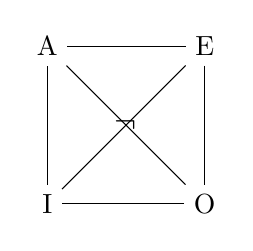
\begin{tikzpicture}[baseline=(A)]
    \node at (0,0) (not) {{\large $\mathbf{\neg}$}};
    \node at (-1,1) (A) {A};
    \node at (1,1) (E) {E};
    \node at (-1,-1) (I) {I};
    \node at (1,-1) (O) {O};

    \draw (A) -- (O);
    \draw (E) -- (I);
    \draw (A) -- (E) -- (O) -- (I) -- (A);
  \end{tikzpicture}
  \begin{minipage}[t]{.69\linewidth}
    The \textit{Square of Opposition} places the 4 statements at the vertices of a square as shown, and claims that diagonally opposite statements are contradictory, i.e. negations of each other.

    Using your predicate logic expressions from the previous part, justify how A contradicts O, how E contradicts I, and vice versa. Provide precise derivations using rules of logical equivalence.
  \end{minipage}
  
  \begin{solution}\\
    Applying negation on A: \\
    1: $\neg (\forall x (S(x) \implies P(x)))$\\
    2: $\exists x \neg(\neg S(x) \lor P(x))$ conditional-disjunction equivalence and demorgan's law \\
    3: $\exists x (S(x) \land \neg P(X))$ demorgan's law\\
    This matches the expression of O. Hence proven A contradicts O and vice versa\\\\
    Applying negation on E:\\
    1: $\neg (\forall x (S(x) \implies \neg P(x)))$\\
    2: $\exists x \neg(\neg S(x) \lor \neg P(x))$ conditional-disjunction equivalence and demorgan's law\\
    3: $\exists x (S(x) \land P(X))$ demorgan's law \\
    This matches the expression of I. Hence proven E contradicts I and vice versa
  \end{solution}
  \end{parts}
  
\end{questions}

\end{document}

%%% Local Variables:
%%% mode: latex
%%% TeX-master: t
%%% End:
